\documentclass[conference,compsoc]{IEEEtran}
% *** CITATION PACKAGES ***
%
\ifCLASSOPTIONcompsoc
  % IEEE Computer Society needs nocompress option
  % requires cite.sty v4.0 or later (November 2003)
  \usepackage[nocompress]{cite}
\else
  % normal IEEE
  \usepackage{cite}
\fi
\usepackage{graphicx}
\graphicspath{ {../} }
\usepackage{amsmath}
\usepackage{url}
\interdisplaylinepenalty=2500
\usepackage{array}
\usepackage{tikz}
\usepackage{listings}
\usepackage[font=footnotesize]{caption}
\usetikzlibrary{positioning}
\newcommand{\subparagraph}{}
\usepackage{titlesec}
\setcounter{secnumdepth}{4}
\setcounter{tocdepth}{4}
\setcounter{secnumdepth}{4}
\titleformat{\paragraph}
{\normalfont\normalsize\bfseries}{\theparagraph}{.8em}{}
\titlespacing*{\paragraph}{0pt}{0ex}{0ex}

\begin{document}
\title{Batch Image Processing of Images in a Folder with Python}
\author{\IEEEauthorblockN{Hakan Bostan}
\IEEEauthorblockA{Technical University of \L{}\'{o}d\'{z}\\
\L{}\'{o}d\'{z}, Poland\\
Email: hbostann@gmail.com}}

% make the title area
\maketitle

\begin{abstract}
In this report I will explain the python program developed to batch process images
inside a folder. Program relies mostly on external \textit{SciPy}, \textit{Numpy} and
\textit{Scikit-image} packages. Program accepts the path to the images and an operation
to perform on those images. Operations are not only limited to built-in functions as user
created scripts can also be used to process the images.

\end{abstract}

\section{Introduction}
Image processing is used to carry out many tasks, such as interpretation of medical images or inspection/sorting of products. This processing should be done in the fastest way possible to extract relevant and useful information out of images. Currently there are quite a few software (e.g. Adobe Photoshop, ImBatch) to batch process images. These solutions usually use built-in methods to process the images.

In this program I tried to create a batch image processor which gives the users the freedom of executing their own processes on images while keeping the general properties of a batch image processor. Program is created using Python2.7 and uses some external libraries. 

\section{Method}
The program is written using Python2.7. It also requires \textit{SciPy}, \textit{Numpy} and
\textit{Scikit-image} packages alongside built-in ones to function properly. Program accepts the path to image files to be processed and the operation to be performed on them with options further specifying the operation. Users can also provide their own scripts as operations if needed. After the execution processed images are saved into a new folder called 'output' at the given path.

\subsection{Implementation}
Program can be run from command-line by providing appropriate options. It first uses \texttt{argparse} module to check if the provided data is valid and sufficient enough to carry out requested operation. There are 5 main and  3 optional arguments.
\begin{description}
\item [help] Prints the help text for the command and exits.
\item [list] Prints the built-in operations that can be readily used and exits.
\item [path] Used to pass in the path to the images to be processed.
\item [operation] Used to define which operation should be performed. Cannot be used with \texttt{script}.
\item [script] Used if user wants to execute their own script. Cannot be used with \texttt{operation}.
\item [\textit{value}] Optional. Used to pass in a integer value.
\item [\textit{point}] Optional. Used to pass in coordinates.
\item [\textit{shape}] Optional. Used to pass a structuring element.
\end{description}

For program to work properly, given path should exist. If a built-in operation is chosen program searches for it inside \texttt{scripts} folder, confirms it exists and assigns it to be the function to be used. If a custom script is to be used, it searches the function inside the given script file and assigns it to be the function to be used. Moreover if optional values are also passed it modifies the way the function is called accordingly.

After input validation it creates a new folder called \texttt{output} inside the given director, then it starts to process images. During processing program loads an image to memory, turns it into a 2D image if it is not already and passes it to the processing function determined by the user. Return value of the function is then saved inside the created output directory.

\subsection{Scripts}

\subsubsection{Built-In Scripts}
Each built-in operation is a different python script with only a single function with the same name inside. These functions needs to be the same name with the actual file because the program searches the namespace for the requested operation and uses \texttt{getattr} function call to access the function.

\subsubsection{User Created Scripts}
User created scripts should also be similar to built-in ones. There should only be a single function with the same name of the script file. Function must have an argument to receive the image (in numpy ndarray format) alongside optional arguments. Return value should also be a numpy ndarray which can be interpreted as an image.
\section{Results}
The program is tested with all the built-in functions. To test the user provided scripts, a script file from the script directory is simply removed and used as a user created script. Below are some results of the program run with different operations.

\begin{minipage}{0.48\linewidth}
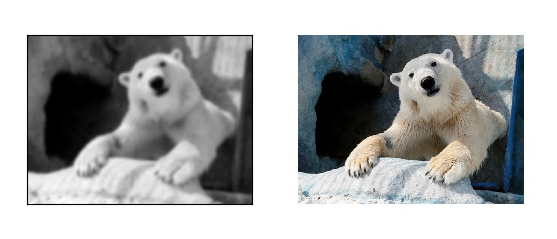
\includegraphics[scale=.5]{Untitled.png}
\captionof{figure}{Result of gaussian blur on left, original on right}
\end{minipage}


\begin{minipage}{0.48\linewidth}
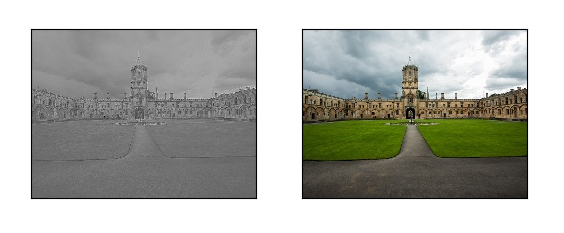
\includegraphics[scale=.5]{Untitled2.png}
\captionof{figure}{Result of sharpening on left, original on right}
\end{minipage}


\begin{minipage}{0.48\linewidth}
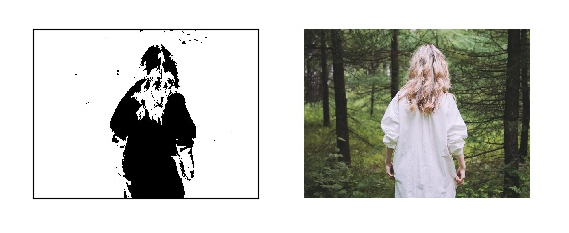
\includegraphics[scale=.5]{Untitled3.png}
\captionof{figure}{Result of region growing on left, original on right}
\end{minipage}


\section{Discussion}
Program works as wanted but there is still a lot to improve. In the current situation program is not user friendly. This can be improved by implementing a GUI. Also algorithms used in some operations, for example \texttt{regionGrowing}, are really inefficient. These can also be implemented in a more efficient way. Overall this program can process images in a directory rapidly and present the output.

\section{Project Materials}
All of the material used in this project is available under \url{https://github.com/hbostann/ImageProcessingProject}.
It includes the ReadMe file, source code for the main program, operation scripts and sample images used for testing.

\pagebreak
%\begin{thebibliography}{1}
%\bibitem{TowAIComp}
%Girod, Bernd, \emph{Leland Stanford Junior University EE368 Digital Image Processing Lecture Notes}
%\end{thebibliography}
\end{document}
